% !TEX encoding = UTF-8 Unicode
\documentclass[12pt,oneside]{memoir}
\usepackage{geometry}
%\geometry{letterpaper}
\geometry{a4paper}
\usepackage{graphicx}
\graphicspath{ {../../img/} }

%% For highlight ranges of text marked with inspector comments
\usepackage{soul}

\usepackage{xcolor}
\usepackage[
    colorlinks=true,
    urlcolor=blue,
    linkcolor=blue,
    citecolor=blue,
    filecolor=blue,
]{hyperref}
\usepackage{memhfixc}
\usepackage{natbib}
\setcitestyle{authoryear,open={(},close={)}}


\setcounter{page}{1}
\pagenumbering{roman}

\title{Introduction: Resurgence of the People}
\author{Sam Popowich}
\date{2020-09-20}

\usepackage{palatino}

\begin{document}

\maketitle
\clearpage

\newpage
\setcounter{page}{1}
\pagenumbering{arabic}

\mainmatter

Introduction and sign-posting.

\section*{Two Canoes}

Two contrasting artworks indicate the rich diversity of Canadian life, and the vastly different interpretations available of the same political experience. In 1995, in the middle of Canadian debates around multiculturalism, Quebec nationalism, and Indigenous sovereignty, James Tully’s book on modern constitutionalism, \emph{Strange Multiplicity}, drew inspiration from Haida artist Bill Reid’s sculpture, \emph{The Spirit of Haida Gwaii}. The sculpture depicts a crew of diverse beings drawn from Haida culture and the European encounter paddling a canoe, “squabbling and vying for recognition” \citep[24]{Tully1995}. Tully makes Reid’s crowded canoe a “symbol of the age of cultural diversity” (24) and a metaphor for the pluralistic society of that Tully considers a “genuinely post-imperial age” (17) following the collapse of the Soviet Union and the apparent triumph of liberal-democratic constitutionalism.

The passengers in Reid’s canoe are gathered around a central figure, “holding the speaker’s staff in his hand… the chief or exemplar, whose identity… is uncertain” (18). For Tully, the chief’s position is one of mediation or reconciliation, just as liberal philosophy has been, since Locke, one of tolerance, pluralism, and the peaceful mediation of competing interests. However, in the twenty-five years since Tully’s book was written, the pacific horizons of liberal constitutionalism have become increasingly fraught. The continuation of settler-colonial violence, not least in the Murdered and Missing Indigenous Women and Girls (MMIWG) crisis in Canada, as well as the resurgence of right-wing fundamentalism, populist governments, the reinstatement of intolerance and oppression baed on race, gender, class, and disability - all in the context of social and economic crisis - all serve challenge Tully’s interpretation of Reid’s sculpture. In a world of Donald Trump, Boris, Johnson, Jair Bolsonaro, and others, it is hard for us now to take Tully’s description of the chief seriously: “listen[ing] attentively to each [passenger], hoping to guide them to reach an agreement, without imposing a metalanguage or allowing any speaker to set the terms of the discussion” (24). 

In the face of the ongoing crises of civil society, it is tempting to reject Tully’s liberal conception of sovereignty and opt instead for a Hobbesian model of intersubjective war limited only by the power of Leviathan. But this choice is a false one, as Hardt and Negri suggest at the beginning of \emph{Empire}, published five years after \emph{Strange Multiplicity} in the wake of the 1999 anti-globalization protests. There is a third constitutional option, one which is often dismissed out of hand because, as we will see, it relies upon an immanent, unruly creativity, a self-directed activity that does not rely on the calm wisdom of a leader, and therefore poses a challenge both to the Lockean and Hobbesan constitutional orders. This third option can be seen in a contemporary artwork that echoes and challenges \emph{The Spirit of Haida Gwaii} in many ways.

Kent Monkman is a two-spirit Cree artist born in Ontario and raised in Winnipeg, Manitoba. Monkman’s paintings have struck a chord with their provocative “reconfigurations” of classical European forms, motifs, and images in the service of challenging the settler-colonial artistic heritage on which today’s settler-colonialism relies \citep{Elston2012}. Echoing Tully’s understanding of “hidden constitutionalism” surviving within dominating, hegemonic institutions, Monkman’s work recognizes the continuation of Indigenous identity and politics within an artistic tradition that has tended to erase Indigeneity in favour of settler-colonial triumph. 

Monkman’s 2019 painting, \emph{Resurgence of the People}, depicts, like Reid’s sculpture, a crowded canoe; only in this instance, Monman appears to reject Tully’s conciliatory understanding of the politics of recognition in favour of a self-affirmation of the multitude in all its diversity. In Monkman’s canoe, while there is still a visually central figure, the “passengers” (the term seems inappropriate here) are not gathered around pressing their case for recognition. Rather, the canoe is filled with people of colour of various ages and genders, all looking after one another, not in a struggle for recognition, but in decentered, mutual support and care, opening up a conception of politics broader than the democratic constitutionalism which is Tully’s focus. 

This alternative perspective, a rejection of both Hobbes’ and Locke’s conceptions of sovereignty, is made explicit by the central figure of Monkman’s painting. Gone is the enigmatic chief who “must act like a mother in caring for the common good if s/he is to secure respect and authority” \citep[25]{Tully1995}. The need to secure respect and authority is a remnant of the false choice, a holdover of the need for constitutional sovereignty and centralization. In \emph{Resurgence of the People}, Reid’s chief has been replaced by Monkman’s wild and exuberant alter-ego, Miss Chief Eagle Testickle, “a time-traveling, shape shifting, supernatural being who reverses the colonial gaze to challenge received notions of history and Indigenous peoples” \citep{MonkmanBiography}.

While Reid’s chief accords or grants recognition to the passengers in the canoe, indicating the accommodation of diverse identities within a hierarchical sovereign constitution, Miss Chief offers her own exuberant affirmation, overflowing the limits of the canoe and suggesting an irrepressible power that does not depend either on recognition, authority, or a constitution. Similarly, the others in the canoe are not looking to Miss Chief for recognition or leadership, but are living their lives, helping each other without concern for constitutional niceties, but all fully aware that they are living in the same boat. While Tully sums up Reid’s canoe as “go[ing] on forever anchored in the same place” \citep[33]{Tully1995}, betraying the desire of liberal politics for an orderly, predictable, and risk-free future, Monkman’s canoe is thrusting powerfully forward through choppy and uncertain seas. There is an unbridgeable gulf between the self-determining forward motion of Monkman’s canoe and the static rockbound impotence of settler-colonialism. The resurgence of the people is their unruly momentum, produced by the determined paddling of Indigenous men and women, unconstrained by the power of a constitution, a momentum that turns away from the white, patriarchal capitalist state to make its own way in the world.

Miss Chief does not need anyone’s recognition; rather, it is the white men stuck on the rock with their weapons who clamour for recognition: of their authority, their power, their capacity for violence. The new politics of identity differs from the older politics of recognition precisely in this insistence on self-affirmation that transcends a universal, egalitarian conception of rights and a procedural, discursive conception of democratic process. It takes seriously the incommensurable, the irreconcilable, and the non-dialectical tensions, antagonisms, and contradictions of contemporary social relations. This insistence challenges hegemonic ideas of the state, of democratic participation, of liberty, and of citizenship, all of which play out in current controversies and debates within Canadian society, including Canadian librarianship. 

\bigskip

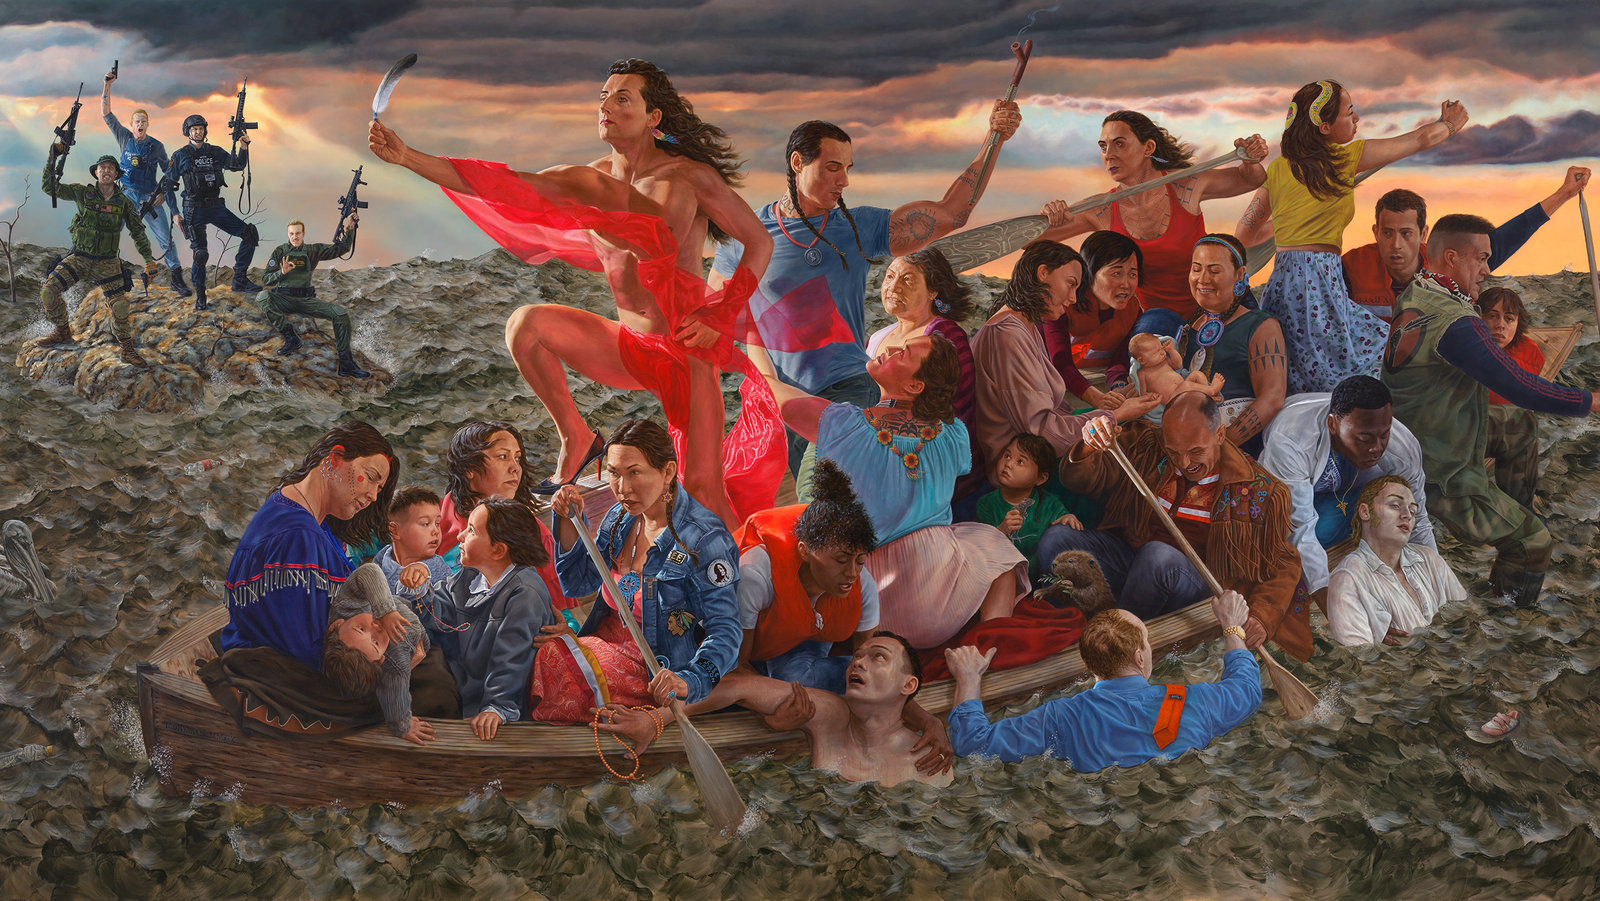
\includegraphics{resurgence}

\bigskip
\begin{flushleft}
Kent Monkman, \emph{Resurgence of the People} (2019)
\end{flushleft}

\bigskip

Tully’s interpretation of \emph{The Spirit of Haida Gwaii} exemplifies a common way of looking at Canadian politics that is idealistic in both the philosophical and colloquial meanings of the word. The interpretation is shared by Pierre Elliott Trudeau’s “just society” (first expressed in his bid for the leadership of the Canadian Liberal Party in 1968) and by Justin Trudeau’s promise of “sunny ways” following his election as prime minister in 2015. The Liberals are often seen as “Canada’s Natural Governing Party” at least in part because of this idealism: like Reid’s chief, they help us navigate the tensions and contradictions of Canadian society better than either the conservatives to the right or the New Democratic Party to the left. They secure respect and authority by caring for the common good in a way the conservatives and the NDP cannot.

But Canadian politics is idealistic also in the philosophical sense, seeing ideas and values as self-generating and constituting the foundation of the social if not the natural world. For some Canadian political philosophers like Charles Taylor, the debt to idealism (particularly the work of Hegel) is explicit \citep{Sibley2008, Meynell2011}. For others, like James Tully, it is less pronounced. However, Tully’s practice of public philosophy can be understood in Wittgenstein’s terms as an idealistic “struggle against the bewitchment of our understanding by the resources of language” (\cite[52]{Wittgenstein2009}, \cite[70]{Tully2008}).

The goal of public philosophy, for Tully, is to “free ourselves from… the assumption that our way of political life is free and rational only if it is founded on some form of critical reflection” \citep[39]{Tully2008} in order to expose the conventionality of traditional political perspectives and open up a wider horizon of political possibility. But while grounding his critical public philosophy in concrete practices (of thought, language, and action), Tully retains an idealistic commitment. Once freed of our reliance on critical reflection as a transcendental or foundational ground of philosophizing, Tully writes, “we are now able to see the enlightening multiplicity of conceptions of critical reflection available to us” and “to use these reflective concepts as their grammar manifestly guides us in innumerable ways to do: not to provide foundations for, but to reflect critically on our well-trodden ways of thought and action, rendering them less indubitably foundational, and thereby disclosing possibilities of thinking and acting differently” \citep[70]{Tully2008}.

This kind of idealism - the replacement of one set of (erroneous) ideas with better ones - is precisely the idealism of the Young Hegelians Marx and Engels critiqued in The German Ideology. For Marx and Engels, the idealistic view that “the relations of men, all their doings, their fetters and their limitations are products of their consciousness”, emancipatory or progressive philosophy consists simply of exchanging one consciousness for another \citep[36]{MarxEngels1976}. Compare this with Wittgenstein’s insistence that “a picture held us captive” \citep[53]{Wittgenstein2009}. In the Marxist tradition, it is not language or ideas or pictures that hold us captive, but real material relations between human beings that are not contingent but necessary due to the unchangeable nature of history itself.

Indeed, language, ideas, and political philosophy itself, in the Marxist view, are produced by these material and social relations, and this raises the question of Canadian political philosophy to the realities of Canadian politics and history. Can the social philosophy of Taylor and the constitutional theory of Tully be understood in terms not only of responding to particular political challenges (Indigenous and Quebecois sovereignty, for example) - which both Taylor and Tully explicitly recognize - but also as deriving as legitimating the positions and actions taken by the Canadian state?

The political and constitutional problems raised by confederation, and which generations of Liberal politicians have believed could be resolved at the political level, have proven intractable. In September 2020, Sipekne'katik First Nation launched a Mi’kmaq-regulated lobster fishery in Nova Scotia, claiming a treaty right that goes back to the 1760s \citep{Palmater2020}. Settler-Canadian members of the commercial fishing industry have threatened to pull Mi’kmaq lobster traps (which they consider “illegal” because they aren’t governed by state fishing licenses) leading to confrontations between First Peoples and Settlers, “mediated” by the RCMP. The RCMP are legally obliged to protect the Mi’kmaq treaty right, but rhetorically side with the Settlers. In a video clip played on Canadian news channels, one RCMP officer is heard explaining to a white fisherman, “whether we like it or not, they’re allowed to go out and fish”. This us vs. them dynamic in Canadian Settler-Colonial society is one of the problems Taylor’s and Tully’s political philosophy sets out to address. But in the thirty years since Taylor’s essay on the politics of recognition appeared, nothing has really changed in terms of relations between the Settler state, Indigenous peoples, and Quebecois nationalists.

The perseverance of these constitutional questions raises a second important question: if Marxism offers an alternative to the idealist philosophy of Canadian liberalism, can historical materialism offer any alternative strategies or proposals which might stand a better chance of achieving something like Trudeau’s “just society”? Tully justifies comparing Wittgenstein and Habermas in part by arguing that “we come to understand some complex work best by comparing its similarities and dissimilarities with another closely related work” \citep[71]{Tully2008}. In this thesis, then, I will explore the questions raised about the connection between Canadian political philosophy and the recent history of Canadian politics by comparing Taylor’s and Tully’s work with that of Antonio Negri.

Negri is of the same generation as Taylor, and their thought is informed by the social and political changes of the 1960s and the 1970s. Both have written in different ways on the effects of the neoliberal turn (Negri from the perspective of autonomist Marxism; Taylor from the perspective of communitarian liberalism), the question of identity and individualism within larger collective structures, and both engage deeply with an earlier political philosopher, sometimes in novel or anomalous ways (Spinoza for Negri; Hegel for Taylor). Tully, on the other hand, shares with Negri a concern for constitutional questions and imperialism, though their approaches differ in radical ways.

Identity politics is one of the major political issues of the day. It plays a role in right-wing extremism, white nationalism, and authoritarian populism; it plays a role in climate change, where the “anthropocene” or “capitalocene” debate signals a disagreement as to whether responsibility for climate change lies with some people or all people \citep{Moore2016}; and it plays a role in the pandemic response, as we witness a phenomenon believed to be universal (the virus) in fact having differential effects based on class, gender, and race. The social effects of quarantine and lockdown are felt differently by men and women, white people and people of colour. The BlackLivesMatter protests which returned with a vengeance in the summer of 2020, as well as the intersectionality of the police/prison abolition movement, all indicate that the purported universalism of liberal theory - everyone in the canoe placidly agreeing to go in the same direction -  is no longer tenable.

In many ways, today’s resurgence of the people echoes the explosion of post-colonial demands, new social movements, and worker-student solidarity in 1968. As Boltanski and Chiarello note in \emph{The New Spirit of Capitalism}, the ten years between 1968 and 1978 - the ten years in which neoliberalism learned how to deal with the demands of 1968 - were marked by “a social movement on the offensive, extending significantly beyond the boundaries of the working class” \citep[167]{BoltanskiChiarello2005}. The fact that the revolts of 1968 did not constitute the expected (or feared) worker revolution caused a re-evaluation of both liberal and radical political theory. To understand how Taylor and Tully’s political philosophy fits with this dynamic, we must return to the events of 1968.

\section*{1968: A New Kind of Revolution}



For the Marxist critique part, just sketch those into the chapter outline. No need to go into detail here. Include Shoikhebrod and Forrester.


 


\backmatter

\bibliographystyle{plainnat} 
\bibliography{../Bibliography}
\end{document}